\documentclass[12pt]{article}

\usepackage{mathtools}
\usepackage{bm}
\usepackage{dsfont}
\usepackage{comment}
\usepackage{amssymb}
\usepackage{amsmath}
\usepackage{dsfont}
\usepackage{comment}
\usepackage[nomarkers,figuresonly]{endfloat}
\usepackage{amsfonts}

\usepackage{multirow}
\usepackage{graphicx}
\usepackage{caption}
\usepackage{subcaption}
\usepackage{float}
\usepackage[section]{placeins}
\usepackage[font=normalsize,labelfont=bf]{caption}
\captionsetup[table]{font=footnotesize,labelfont={sf}}

\usepackage{booktabs, siunitx}
\usepackage{array}
\usepackage{accents}
\usepackage{setspace}
\usepackage[round]{natbib}
\usepackage[titletoc]{appendix}
\usepackage{lscape}

\usepackage{longtable}
\usepackage{totcount}
\usepackage{alphalph}
\usepackage{tabularx}
\usepackage{rotating}

\usepackage{hyperref} 
\usepackage{fullpage} 
\usepackage{tikz}
\usepackage{pgfplots}
\usepackage{pgfplotstable}
\usetikzlibrary{shapes, arrows.meta, positioning,arrows.meta,
                chains,
                shapes.geometric,
                decorations.pathreplacing, datavisualization.formats.functions
                }

\begin{document}
	


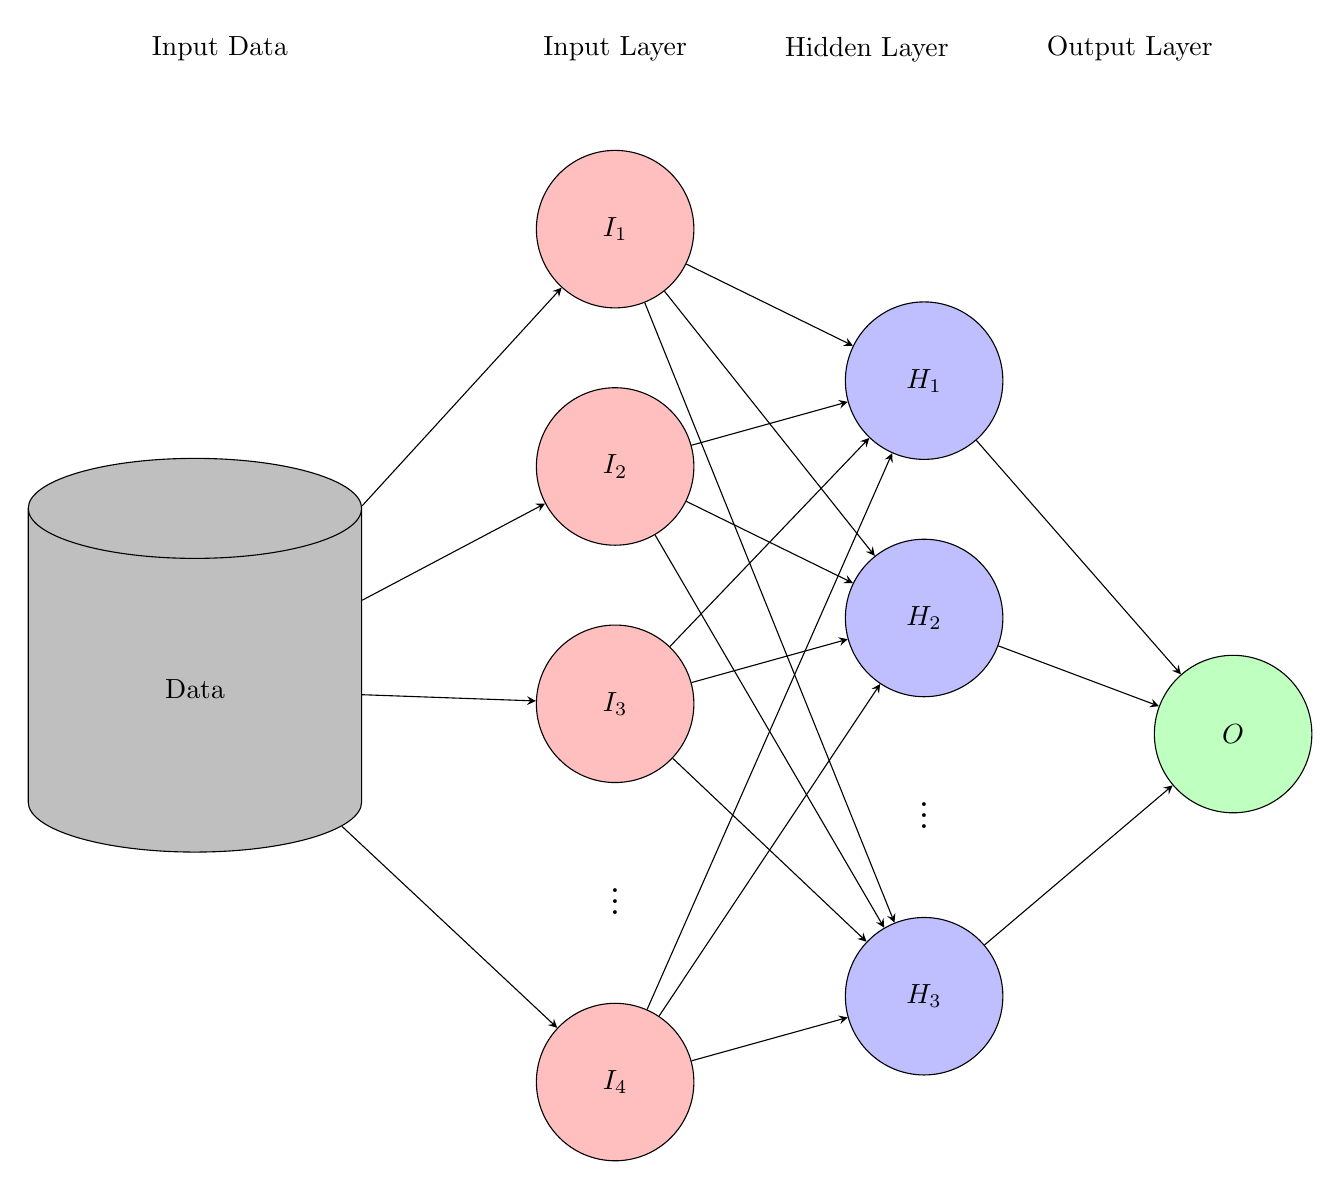
\begin{tikzpicture}[x=1.5cm, y=1.5cm, >=stealth,
every neuron/.style={
circle,
draw,
minimum size=2cm,
fill=red!25
},
hidden neuron/.style={
circle,
draw,
minimum size=2cm,
fill=blue!25
}, 
data/.style={shape=cylinder, draw, shape aspect=0.3,
                shape border rotate=90, minimum height=5cm, text width = 4cm,
                fill=black!25}
                ]


\node[every neuron] (n1) at (0,10){$I_1$};
\node[every neuron] (n2) [below=of n1] {$I_2$};
\node[every neuron] (n3) [below=of n2] {$I_3$};
\node[auto=false] (ell) [below=of n3,]{\Large$\vdots$};
\node[every neuron] (n4) [below=of ell,]{$I_4$};

\node[] (text node) [above= of n1] {Input Layer};
\node[data] (d) [below left=3cm and 2.5cm of n1, align=center] {Data};
\node[] (text node0) [left=3cm of text node] {Input Data};

\node[hidden neuron] (n5) [below right=.5cm and 2.5cm of n1] {$H_1$};
\node[hidden neuron] (n6) [below=of n5] {$H_2$};
\node[auto=false] (ell2) [below=of n6] {\Large$\vdots$};
\node[hidden neuron] (n7) [below=of ell2] {$H_3$};

\node[] (text node2) [right= of text node] {Hidden Layer};

\node[circle, draw, minimum size=2cm, fill=green!25] (n8) [below right=.05cm and 2.5cm of n6] {$O$};

\node[] (text node3) [right= of text node2] {Output Layer};

\draw[->] (n1) -- (n5);
\draw[->] (n2) -- (n5);
\draw[->] (n3) -- (n5);
\draw[->] (n4) -- (n5);

\draw[->] (n1) -- (n6);
\draw[->] (n2) -- (n6);
\draw[->] (n3) -- (n6);
\draw[->] (n4) -- (n6);

\draw[->] (n1) -- (n7);
\draw[->] (n2) -- (n7);
\draw[->] (n3) -- (n7);
\draw[->] (n4) -- (n7);

\draw[->] (n5) -- (n8);
\draw[->] (n6) -- (n8);
\draw[->] (n7) -- (n8);

\draw[->] (d) -- (n1);
\draw[->] (d) -- (n2);
\draw[->] (d) -- (n3);
\draw[->] (d) -- (n4);

\end{tikzpicture}

\newpage 

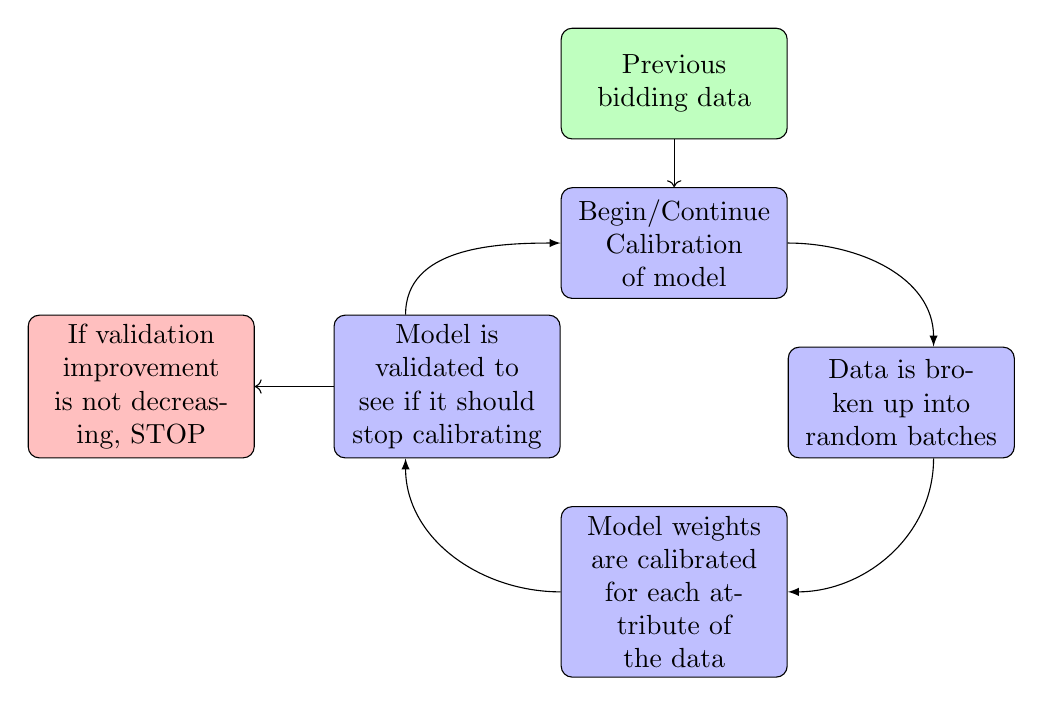
\begin{tikzpicture}[
	node distance=4ex and 0em,
	block/.style={rectangle, draw, fill=white!20, 
		text width=7.5em, text centered, rounded corners, minimum height=4em},
	line/.style={draw, -latex},
	]
	
	\node [block, fill=green!25] (0) {Previous bidding data};
	\node [block, below= of 0, fill=blue!25] (1) {Begin/Continue Calibration of model};
	\node [block, below right= of 1,fill=blue!25] (2) {Data is broken up into random batches};
	\node [block, below left= of 2,fill=blue!25] (3) {Model weights are calibrated for each attribute of the data};
	\node [block, above left= of 3,fill=blue!25] (4) {Model is validated to see if it should stop calibrating};
	\draw [->] (0) -- (1) ;
	\node [block, left = 1cm of 4,fill=red!25] (break) {If validation improvement is not decreasing, STOP};
	\draw [->] (4) -- (break) ;  
	\path [line] (1.east) to[out=0, in=90] (2.60);
	\path [line] (2.-60) to[out=-90, in=0] (3.east);
	\path [line] (3.west) to[out=180, in=-90] (4.-120);
	\path [line] (4.120) to[out=90, in=180] (1.west);
\end{tikzpicture}
	\newpage 
	
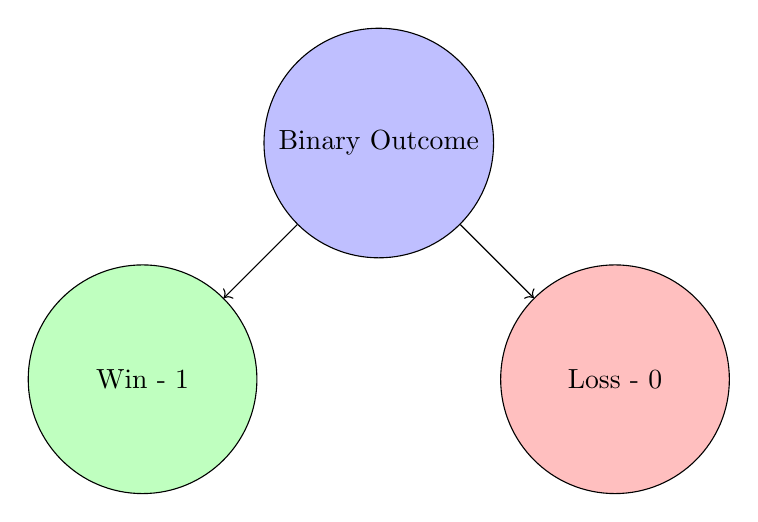
\begin{tikzpicture}[
	node distance=4ex and 0em,
	MyNode/.style={circle, draw, fill=white!20, 
		text width=7.5em, text centered,  minimum height=4em}
	]
	
\node [MyNode, fill=blue!25] (main) at (0,0) {Binary Outcome}; 
\node [MyNode, fill=green!25] (win) at (-3,-3) {Win - 1} ; 
\node [MyNode, fill=red!25] (loss) at (3,-3) {Loss - 0} ; 
\draw [->] (main) -- (win);
\draw [->] (main) -- (loss);

\end{tikzpicture}	

\newpage 
\begin{align*}
	\min \ & c^\top x \\ 
	s.t. \ & Ax = b \\
	& x \geq 0. 
\end{align*}

\newpage 
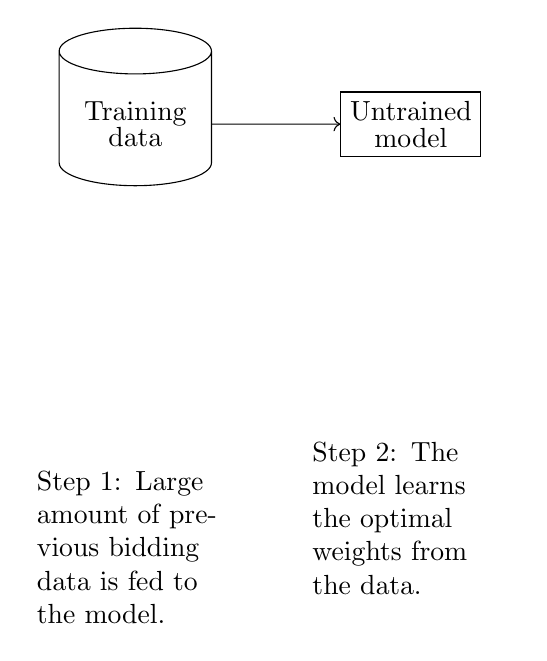
\begin{tikzpicture}[
    node distance = 3.5cm,
    disc/.style = {shape=cylinder, draw, shape aspect=0.3,
                shape border rotate=90,
                text width=17mm, align=center, 
                font=\linespread{0.8}\selectfont,
                minimum height=2cm},
    mdl/.style = {shape=ellipse, aspect=2.2, draw},
    alg/.style = {draw, align=center, font=\linespread{0.8}\selectfont}
                    ]

\node (n1) [disc] {Training\\ data};
\node (n2) [alg, right of=n1]  {Untrained\\ model};
\draw[->] (n1) -- (n2) ;

%\node (n3) [mdl]  {Model};
%\node (n4) [disc] {Test\\ data};
%\node (n3) [mdl]  {Model\\ Validation};
%\node (n3) [mdl]  {Model\\ Shifts};

\node[below=of n1, text width=2.5cm] {Step 1: Large amount of previous bidding data is fed to the model.};
\node[below=of n2, text width = 2.5cm]  {Step 2: The model learns the optimal weights from the data.};


%\path[draw,->] (n1) edge (n2)
 %(n2) edge (n3)
               %(n3) edge (n4)
                    %(otsu.east) -| (right) -- (left) |- (gchannel)
                    %(gchannel) edge (closing)
                    %(closing) edge (NN)
                    %(NN) edge (limit)
                    
    \end{tikzpicture}
    
\newpage 
\begin{align*}
	\min \ & c^\top x \\ 
	s.t. \ & Ax = b \\
	& x \geq 0. 
\end{align*}


\newpage
\begin{tikzpicture}[node distance=3.5cm]
    \draw[shift={(0,0)}, color=black] (0pt,3pt) -- (0pt,-3pt);    
    \draw[shift={(4,0)}, color=red] (0,6pt) -- (0pt, -6pt);
    \draw[shift={(8,0)}, color=green] (0,6pt) -- (0pt, -6pt);
    \draw[shift={(12,0)}, color=black] (0pt,3pt) -- (0pt,-3pt);
    \draw[->, color=green] (8,0) -- (16,0);
    \draw[<-, color=red] (-2,0) -- (4,0);
    \draw[-, color=blue] (4,0)--(8,0);
    \draw (8,-.5) node[below] {100.50}; 
    \node[align=center] at (8,-2) {Winning\\ bid price}; 
    \node[align=center] at (4,2) {Next best\\ bid price \\(Boundary Margin)};
    \draw (4,.65) node[above] {100.25};
    \draw[decorate, decoration={brace, amplitude=10pt}] (4, 3)--(8,3)
     node[black,midway,yshift=1cm, align=center] {Unrealized gain\\(if winner of auction)};
    \draw[decorate, decoration={brace, amplitude=10pt}] (8,.5)--(16,.5)
     node[black,midway,yshift=1cm, align=center] {Winning\\ bids};  
    \draw[decorate, decoration={brace, amplitude=10pt}] (-2,.5)--(4,.5)
     node[black,midway,yshift=1cm, align=center] {Losing\\ bids};   
    
    % \draw (0,-.5) node[below] {$\ldots$};
    % \draw (2,-.5) node[below] {100.00}; 
    % \draw (6,-.5) node[below] {101.00};
    
    % \draw (8,-.5) node[below] {$\ldots$};
\end{tikzpicture}

\newpage 


\begin{tikzpicture}[domain=0:8]
  \draw[very thin,color=gray, step=2cm] (-0.2,-2.1) grid (7.9,7.9);
  \draw[->] (-0.2,0) -- (8.2,0) node[right] {Actual win rate};
  \draw[->] (0,-2.2) -- (0,8.2) node[above] {Estimated win rate};
  \node[color=black] at (2.0, 2.3) {\Large \textbullet};
  \node[color=black] at (4.0, 3.9) {\Large \textbullet};
  \node[color=black] at (6.0, 4.5) {\Large \textbullet};
  \node[color=red] at (2.0, 2.9) {\Large \textbullet};
  \node[color=red] at (4.0, 3.2) {\Large \textbullet};
  \node[color=red] at (6.0, 2.9) {\Large \textbullet};
  
\draw[decorate, decoration={brace, mirror, amplitude=10pt}] (6,2.9)--(6,4.5)
     node[black,midway,xshift=1cm, align=right] {Gap};   

\end{tikzpicture}

\begin{tikzpicture}[domain=0:8]
  \draw[very thin,color=gray, step=2cm] (-0.2,-2.1) grid (7.9,7.9);
  \draw[->] (-0.2,0) -- (8.2,0) node[right] {Actual win rate};
  \draw[->] (0,-2.2) -- (0,8.2) node[above] {Estimated win rate};
  \node[color=black] at (2.0, 2.3) {\Large \textbullet};
  \node[color=black] at (4.0, 3.9) {\Large \textbullet};
  \node[color=black] at (6.0, 4.5) {\Large \textbullet};
  \node[color=red] at (2.0, 2.5) {\Large \textbullet};
  \node[color=red] at (4.0, 3.7) {\Large \textbullet};
  \node[color=red] at (6.0, 4.7) {\Large \textbullet};
  
\end{tikzpicture}
 \newpage 
 \begin{landscape}
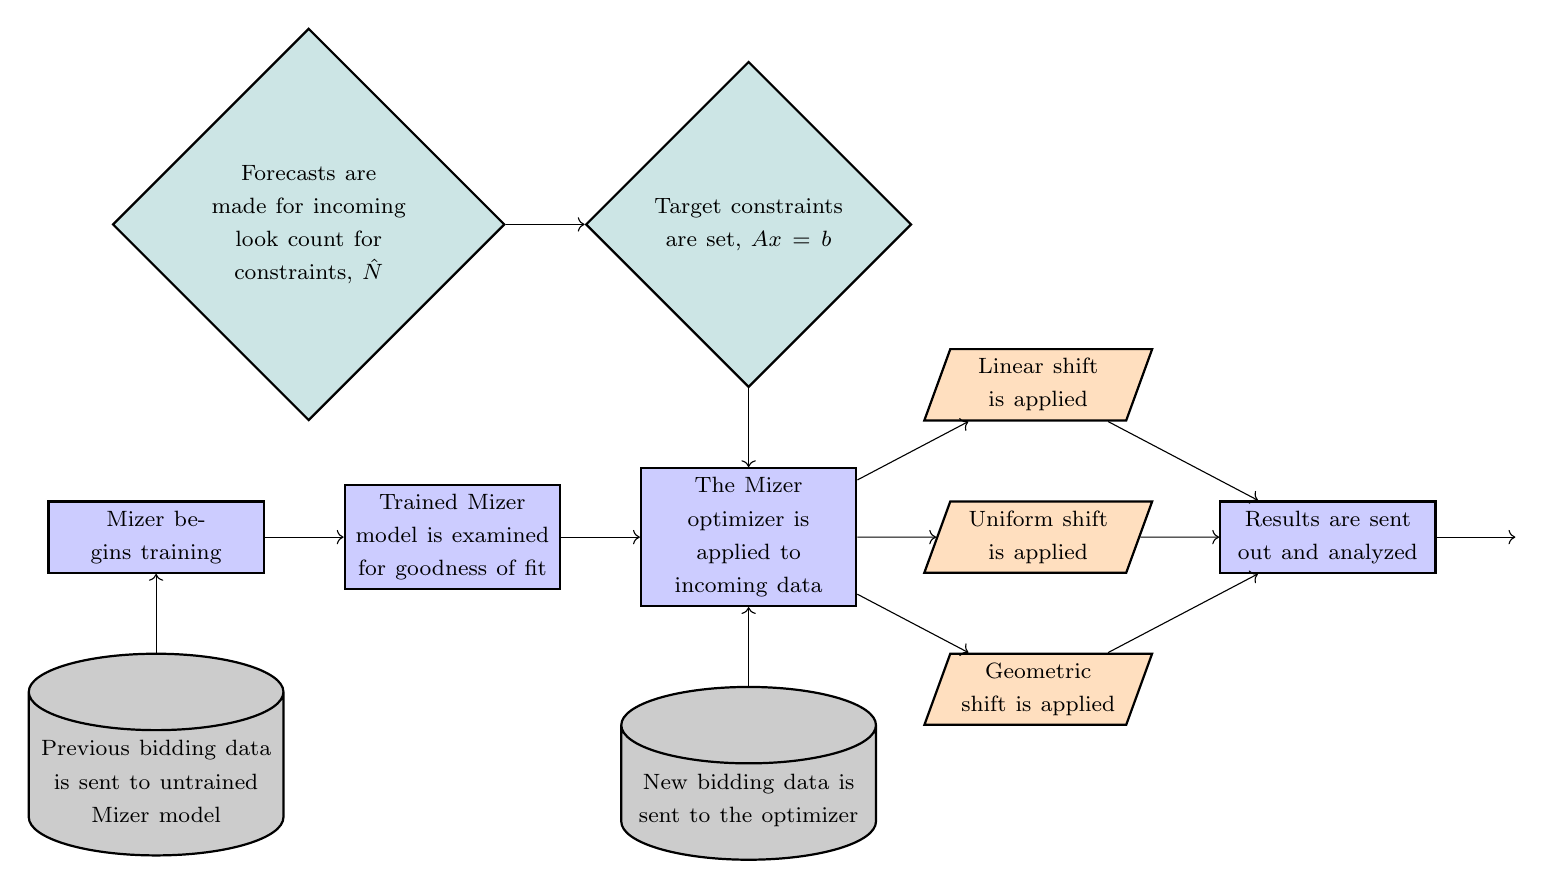
\begin{tikzpicture}
[
MizerNode/.style={rectangle, draw=black, thick,
text width = 2.5cm, align=center, fill=blue!20},
OptionalNode/.style={trapezium,   trapezium left angle=70, 
  trapezium right angle=110, draw=black, thick, 
text width = 2cm, align=center, fill=orange!25},
DataNode/.style={cylinder, draw=black, thick,  
text width = 3cm, align=center, shape border rotate=90, shape aspect=0.3, fill=black!20},
TargetNode/.style={diamond, draw=black, thick, align=center,text width = 3cm,
fill=teal!20}
]

\node[MizerNode] (Training)  {\footnotesize Mizer begins training};
\node[MizerNode] (Trained) [right=of Training]{\footnotesize Trained Mizer model is examined for goodness of fit};
%\node at (12,0) [MizerNode] {Results are analyzed}; 

\node[MizerNode] (Optimizer) [right=of Trained]{\footnotesize The Mizer optimizer is applied to incoming data}; 
\node[OptionalNode] (Uniform) [right=of Optimizer]{\footnotesize Uniform shift is applied};
\node[OptionalNode] (Geometric) [below=of Uniform]{\footnotesize Geometric shift is applied};
\node[OptionalNode] (Linear)[above=of Uniform]{\footnotesize Linear shift is applied}; 
\node[MizerNode] (Results) [right=of Uniform] {\footnotesize Results are sent out and analyzed}; 
\node[DataNode](TrainingData)[below=of Training] {\footnotesize Previous bidding data is sent to untrained Mizer model};
\node[DataNode](EvalData) [below=of Optimizer] {\footnotesize New bidding data is sent to the optimizer};
\node[TargetNode] (Targets) [above=of Optimizer]{\footnotesize Target constraints are set, $Ax=b$};
\node[TargetNode] (Forecasts) [left=of Targets]{\footnotesize Forecasts are made for incoming look count for constraints, $\hat{N}$};
\node[](null)[right=of Results]{};

\draw[->] (Forecasts) -- (Targets);
\draw[->] (Targets) -- (Optimizer);
\draw[->] (Trained) -- (Optimizer);
\draw[->] (Optimizer) -- (Uniform);
\draw[->] (Optimizer) -- (Linear);
\draw[->] (Optimizer) -- (Geometric);

\draw[->] (Geometric) -- (Results);
\draw[->] (Uniform) -- (Results);
\draw[->] (Linear) -- (Results);

\draw[->] (Training) -- (Trained);
\draw[->] (TrainingData) -- (Training);
\draw[->] (EvalData) -- (Optimizer);
\draw[->] (Results)--(null);
\end{tikzpicture} 
\end{landscape}

\newpage 

\begin{tikzpicture}
\begin{axis}[
    axis lines = center,
    xlabel = \(x\),
    ylabel = {\(f(x)\)},
]
\addplot [
    domain=-.1:2,
    samples=100, 
    color=red
]
{-ln(x)};
\addlegendentry{$y=-\log(x)$}
\end{axis}
\end{tikzpicture}



\newpage


\begin{landscape}
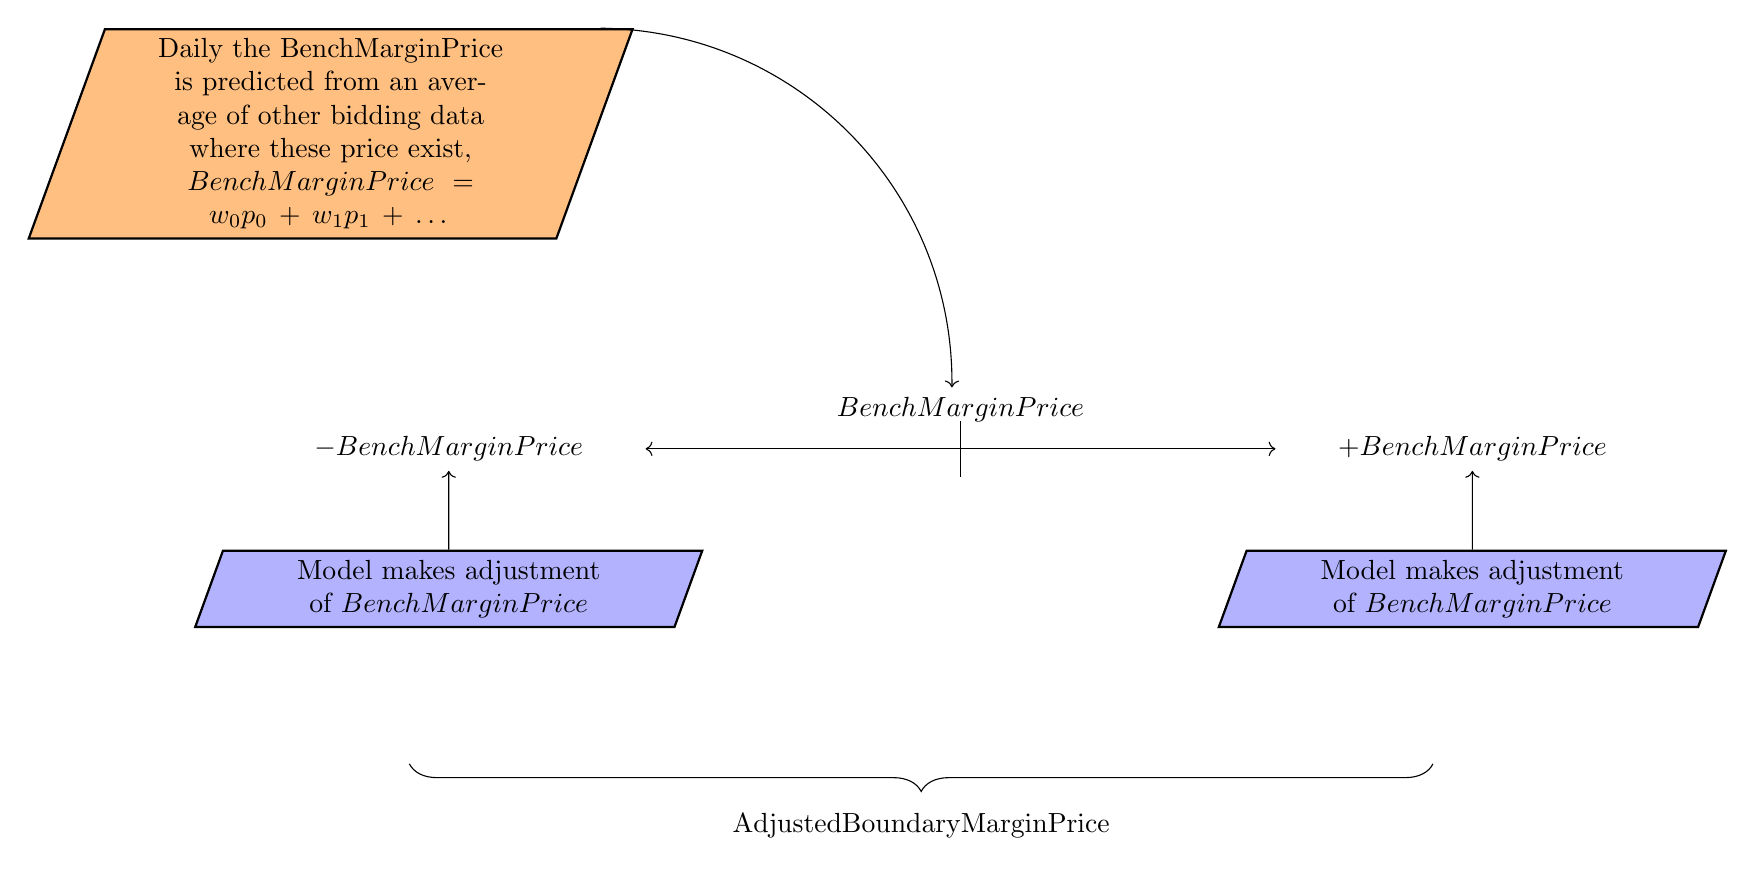
\begin{tikzpicture}
[
flow/.style={trapezium, draw=black,
             fill=orange!50, thick, trapezium left angle=70, 
             trapezium right angle=110, text width=5.5cm, align=center},
model/.style={trapezium, draw=black,
              fill=blue!30, thick, trapezium left angle=70, 
              trapezium right angle=110, text width=5.5cm, align=center}
]

    \draw[shift={(4,0)}, color=black] (0pt,10pt) -- (0pt,-10pt);    
    \draw[<->, color=black] (0,0) -- (8,0);
    \node[flow] (bench) at (-4,4) {Daily the BenchMarginPrice is predicted from an average of other
    bidding data where these price exist,\\ $BenchMarginPrice = w_0 p_0 + w_1 p_1 + \dots $};
    \node[] (null) at (4,.5) {$BenchMarginPrice$};
    \draw[->] (bench) to [bend left=45] (null);
    \node[xshift=-2.5cm] (adj1) at (0,0) {$-BenchMarginPrice$} ;
    \node[xshift=2.5cm] (adj2) at (8,0) {$+BenchMarginPrice$} ;
    \node[model] (negative) [below=of adj1] {Model makes adjustment of $BenchMarginPrice$};
    \node[model] (positive) [below=of adj2] {Model makes adjustment of $BenchMarginPrice$};
    \draw[->] (negative) -- (adj1);
    \draw[->] (positive)-- (adj2);
    \draw[decorate, decoration={brace, mirror, amplitude=10pt}] (-3,-4)--(10,-4)
     node[black,midway, below, align=center, yshift=-.5cm] {AdjustedBoundaryMarginPrice};   
\end{tikzpicture}
\end{landscape} 

 \newpage 
 
 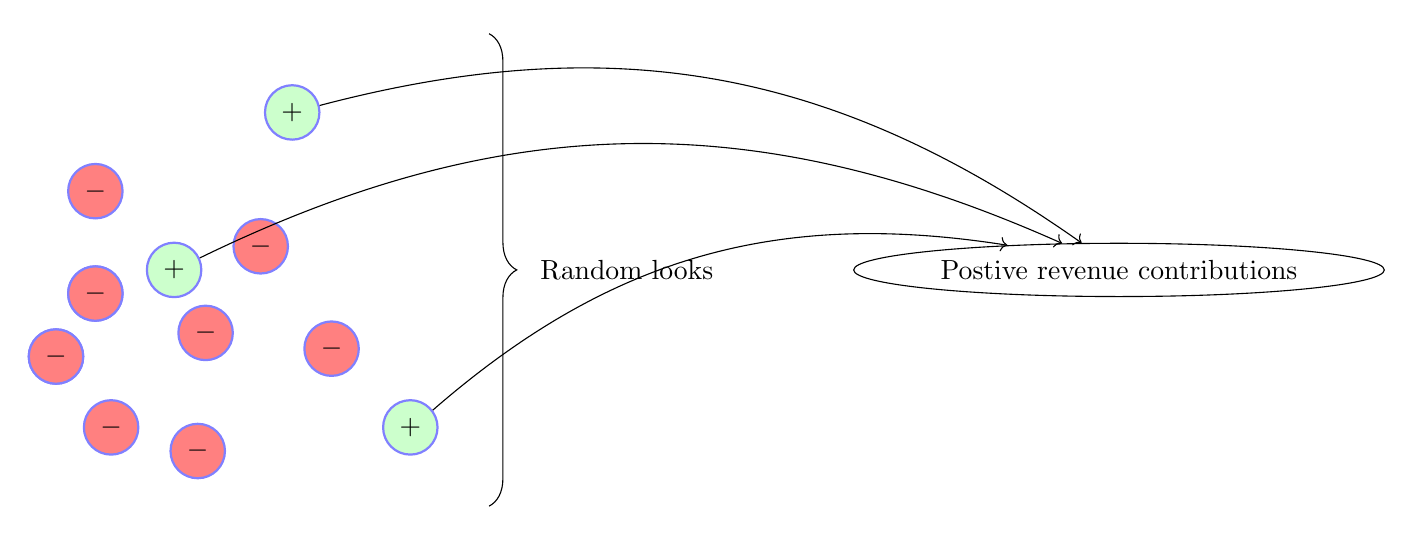
\begin{tikzpicture}
 	  [circ/.style={circle,draw=blue!50,fill=green!20,thick},
 	transition/.style={rectangle,draw=black!50,fill=black!20,thick}]
 	
 	\node[circ](s) at (0,0) {+}; 
 	\node[circ](s1) at (1.5,2) {+}; 
 	\node[circ, fill=red!50] at (-1,1) {$-$}; 
 	\node[circ](s2) at (3,-2) {+}; 
 	\node[circ,fill=red!50] at (1.1,.3) {$-$}; 
 	\node[circ,fill=red!50] at (-1,-.3) {$-$}; 
 	\node[circ,fill=red!50] at (-1.5,-1.1) {$-$}; 
 	\node[circ,fill=red!50] at (.4,-.8) {$-$}; 
 	\node[circ,fill=red!50] at (-.8,-2) {$-$}; 
 	\node[circ,fill=red!50] at (2,-1) {$-$}; 
 	\node[circ,fill=red!50] at (.3,-2.3) {$-$}; 
 	\node[circ,fill=red!50] at (-1,-.3) {$-$}; 
 	\node[circ,fill=red!50] at (-1.5,-1.1) {$-$}; 
 	\node[ellipse, draw] (null) at (12,0) {Postive revenue contributions}
 	edge[<-, bend right=25] (s)
 	edge[<-, bend right=25] (s1)
 	edge[<-, bend right=25] (s2);  	  	
 	 \draw[decorate, decoration={brace,  amplitude=10pt}] (4,3)--(4,-3)
 	node[black,midway, below, align=center, xshift=1.75cm, yshift=.25cm] {Random looks};
 	

 	
 \end{tikzpicture}   


\end{document}